\section{Projet Wikitty}

Wikitty est un projet important chez code lutin, mon travail à été sur un sous
projet de wikitty, et donc pour le comprendre il est important de présenter
le projet Wikitty.


\subsection{Principe}

Ce projet est une base de données orientée documents et API de persistance pour
Java. Il permet d'enregistrer dans une base clé/valeur des objets wikitty, la
clé est un id généré qui est unique pour chaque wikitty. 

Un wikitty possède des extensions et les extensions possèdent des champs nommés
et chaque champ est une clé à laquelle on associe des valeurs. Et des extensions
peuvent dépendre d'autre extension.

Par exemple une extension personne qui possède deux champs : nom et prénon.
Une autre extension ressource qui possède un champs numéro et qui dépends de
l'extension personne. Chaque champs d'extension est défini par son nom et son 
extension par exemple pour notre extension WikittyPersonne ses champs son nommés:
WikittyPersonne.nom et WikittyPersonne.prenom

Si un wikitty possède l'extension ressource alors ce wikitty possèdera les
champs de l'extension ressource et de l'extension employé, puisque ressource
dépends d'employé.

L'api de wikitty prévois un certain nombre d'extension basique, mais tout
l'intéret est que l'on peut créer ses propres extensions, simplement en écrivant
un modèle uml de classe, qui servira ensuite pour générer les classes java
effectives.

Ensuite il suffit de développer son application simplement en utilisant les
classes générées et les passer à un wikitty service pour le stockage sans plus
se poser de question le tout très simplement.

Cette api à été conçue pour supporter les monter en charge et une utilisation
intensive. Elle supporte aussi la recherche par criteria, et par facette.

La recherche par criteria permet de rechercher des wikitty en fonction de leurs
extensions et des valeurs des différents éléments de ces extensions, sans jamais
écrire de sql, on écrit un critère sur le modèle objet. 

Les facettes permettent de regrouper les résultats de recherche par criteria. 

Tout wikitty posséde un numéro de version, qui évolue en fonction des
modifications faites dessus. L'api prévois que l'on puisse restaurer une version
ciblé d'un wikitty.
%quand wikitty version sera mieux gérer en parler.

\subsection{Existant}

Wikitty sert de base de donnée pour une partie des applications de l'entreprise,
puisque il permet une grande flexibilité. Dès lors ou on peut modéliser les
données en objet on peut les stocker dans avec Wikitty.

Actuellement Wikitty peut être déployé localement, pour une base de données
d'une application, mais il peut être déployé sur un serveur et interrogé grâce
au protocole de communication hessian ou au framework cajo.

Hessian est un protocole de communication pour web service, et cajo est un
framework pour les communications d'application java réparties. 

Une partie des projets actuel de Code Lutin utilise un stockage Wikitty, 
l'objectif est à la généralisation de cette solution pour les projets de 
Code Lutin.

\subsection{Utilisation}

A l'utilisation pour créer ses propres wikitty il faut écrire un diagramme de
classe grâce à l'outil argouml, et que chaque classe porte le stereotype
<<Entity>>, et remplir les différents attribut des classes avec les types
reconnus par java. 

Le fait de stereotyper correctement permet ensuite aux générateurs de générer
les classes java correspondante, et s'assurer qu'elles puissent être stocker
ensuite par Wikitty.

Le déploiement ensuite passe par des fichiers configuration qui permettent la
mise en place des différentes couche de service nécessaire au bon fonctionnement
on peut choisir ainsi d'avoir une base de donnée embarquée ou d'utiliser un
Wikitty service distant.

Celà sans écrire le moindre sql, pour faire des recherches il suffit d'écrire
ses criterias, qui peuvent être construit à partir d'objet wikitty, par exemple 
on veut des wikitty qui ressemble à un modèle, on génère les criterias à partir
de ce modèle.

C'est une approche tout objet, tout java, on se concentre sur l'écriture du code
métier et pas sur l'écriture des couches basses. Puisque le service permet la
sauvegarde, restauration, et recherche.

% Ensuite il suffit d'avoir la base de déployée, et d'utiliser l'interface
% wikittyProxy qui offre les services pour les requêtes de wikitty, les
% sauvegardes, restauration de wikitty. La base de donnée est totalement déléguée
% au wikittyService, pas besoin d'écrire du sql.
% 
% Rajouter que on se sert de wikitty service
% 
% mécanisme de wikitty service et de fichier de propriété liée et tout ça


\subsection{WikittyService, WikittyProxy et WikittyServiceFactory}

Le WikittyService est une interface qui permet de sauvegarder, rechercher,
récupérer des wikitty, il existe des implémentations de service pour différente
base de données, pour des services à distance. Tout les services n'implémentent 
pas toutes les méthodes, par exemple la gestion des authentifications ou la 
gestion d'un cache sont à la charge d'implémentation particulière. Et les
services sont disposés en couche successives pour s'occuper de certain aspect
et déléguant les autres aspect à la couche suivante comme on peut le voir sur 
la figure \ref{pileService}.
%ce n'est pas pas un pattern de chain of responsability

%schéma d'encapsulation de wikitty service
\begin{figure}[!ht]
  	%[height=12cm,width=15cm]
\centering
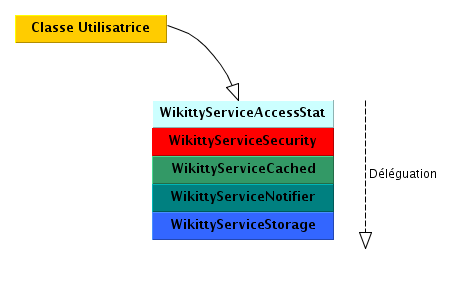
\includegraphics[height=5cm,width=8cm]{image/pileService.png}
  		\caption{Couche de Wikitty Service}
  		\label{pileService}
\end{figure}

La WikittyServiceFactory est une factory au sens pattern, c'est à dire qu'a 
partir de fichier de propriété elle construit et retourne les WikittyServices 
demandé, c'est elle aussi qui organise les couches de service en fonction de ce 
qui est défini dans les fichiers de propriétés.

%exemple de fichier de propriété

Un extrait de fichier de propriétés avec les couches de wikitty service:
\begin{verbatim}
wikitty.WikittyService.components=\
org.nuiton.wikitty.services.WikittyServiceStorage,\
org.nuiton.wikitty.services.WikittyServiceNotifier,\
org.nuiton.wikitty.services.WikittyServiceCached,\
org.nuiton.wikitty.services.WikittyServiceSecurity,\
org.nuiton.wikitty.services.WikittyServiceAccessStat,\
org.nuiton.wikitty.services.WikittyServiceCajoServer
\end{verbatim}

Les propriétés ne sont pas directement manipulé, on se sert d'un object 
ApplicationConfig qui permet de gérer différent niveau de propriétés,
avec des propriétés par default si tout n'est pas défini.

Le WikittyProxy est une surcouche qui encapsule un wikitty service et cache 
certaines complexités pour finalement offrir plus de méthodes et des méthodes 
plus simple. Par exemple l'interface WikittyService ne propose que des 
restore de liste de wikitty, alors que le proxy propose des restore de resultat
unique. Dans le cas d'une session ou l'on s'authentifie auprès d'un wikitty 
service, dans ce cas on récupère un jeton, c'est le proxy qui se charge 
d'injecter le jeton dans chaque demande auprès du Service.


